% Autor: Gabriel Góes Rocha de Lima
% Descrição: Resumo do postesr para o II workshop Inteligência Artificial e Geociências
\documentclass[11pt]{article} % declaração do tipo de documento
\usepackage[utf8]{inputenc} % declaração do tipo de codificação
\usepackage{amsmath} % Para melhor suporte a símbolos matemáticos
\usepackage{ragged2e} % Texto justificado
\usepackage{indentfirst} % pacote para indentação do primeiro parágrafo
\usepackage{setspace} % pacote para definição de espaçamento
\usepackage{titlesec} % Pacote para formatação de títulos
\usepackage{fancyhdr}
\usepackage{geometry} % pacote para definição de margens
\usepackage{graphicx} % pacote para inclusão de imagens
\usepackage{changepage} % pacote para ajustar margens
\usepackage{lipsum} % pacote para geração de texto aleatório
\usepackage{tabularx} % pacote para criação de tabelas
\usepackage{float} % pacote para posicionamento de figuras
\usepackage{array} % pacote para criação de tabelas
\usepackage{multirow} % pacote para mesclar células em tabelas
\usepackage{multicol} % pacote para mesclar colunas em tabelas
\usepackage{caption} % pacote para formatação de legendas


\geometry{
    a4paper,
    left=2cm,
    right=2cm,
    top=1cm,
    bottom=4.5cm
} % definição das margens
\geometry{includehead}
\onehalfspacing % espaçamento de 1.5
\setlength{\parindent}{1.25cm} % indentação de 1.25cm
\setlength{\parskip}{0.5em} % set distance spacing between paragraphs

\begin{document} % início do documento
% Cabeçalhos e rodapé
\pagestyle{fancy}
% adiciona header na primeira página

\fancypagestyle{plain}{
    \fancyhf{} % clear all header and footer fields
    % Configura o cabeçalho esquerdo
    \lhead{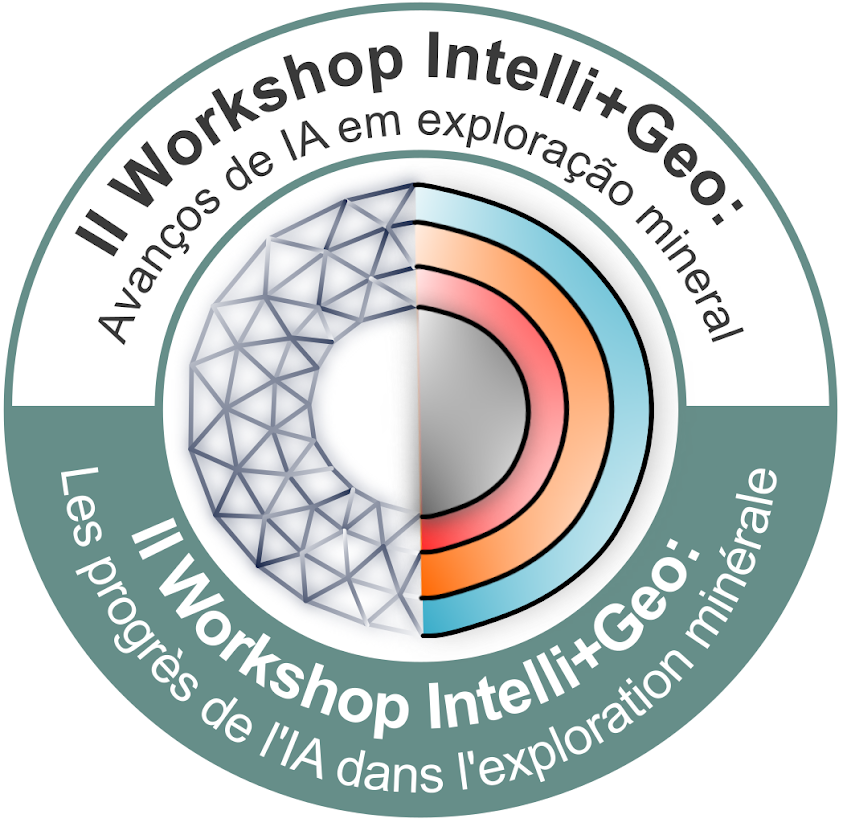
\includegraphics[scale=0.1]{./logo.png}}

    % Configura o cabeçalho direito
    \rhead{\raisebox{1.5cm}{
        \textbf{II Workshop Intelli$^{+}$Geo Avanços de IA em Exploração Mineral}
        }
    }

    % Configura cabeçalho central
    \chead{
        \raisebox{0.75cm}{
            \textbf{28 de fevereiro de 2024}
        }
    }
% RODAPÉ
% -----------------------------------------------------------------------------
%   Organnização/Organisation                       Patrocinadores/Sponsors
%   -------------------------                       ----------------------- #Page
%   logo.png     logo2.png                          logo3.png   logo4.png  

    \cfoot{
        \rule{\textwidth}{0.4pt}
        \vspace*{-0.75cm} 
        \begin{multicols}{2}
            \begin{flushleft}
                \center Organnização / \textit{Organisation}\\
                \vspace{-0.5cm} 
                \center \rule{0.25\textwidth}{0.4pt}\\
                \vspace{0.1cm} 
                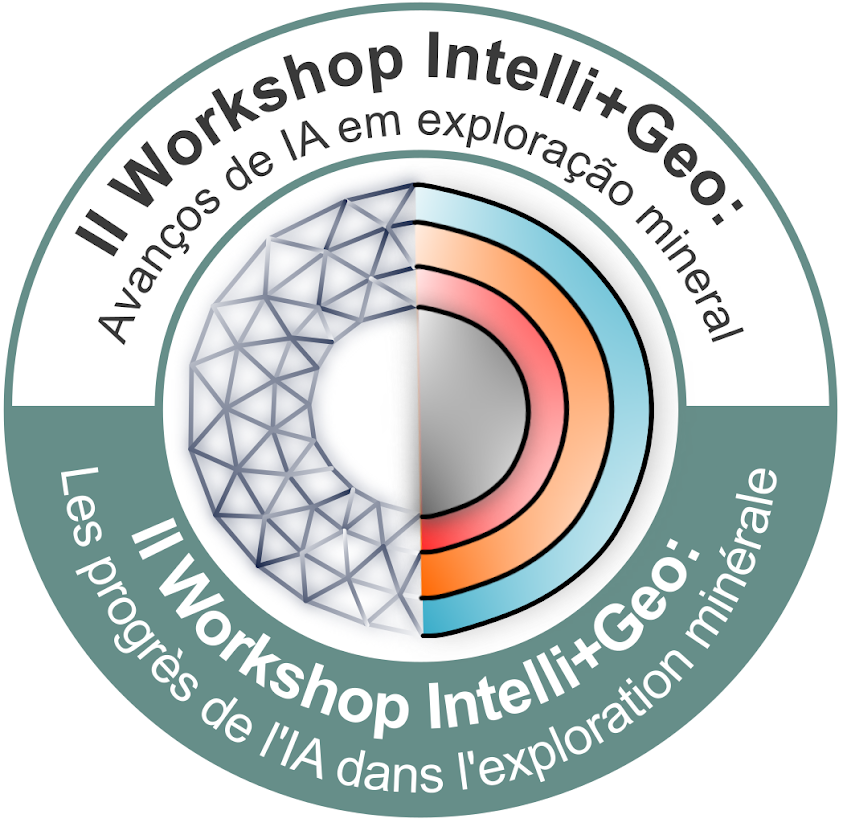
\includegraphics[scale=0.05]{./logo.png}
                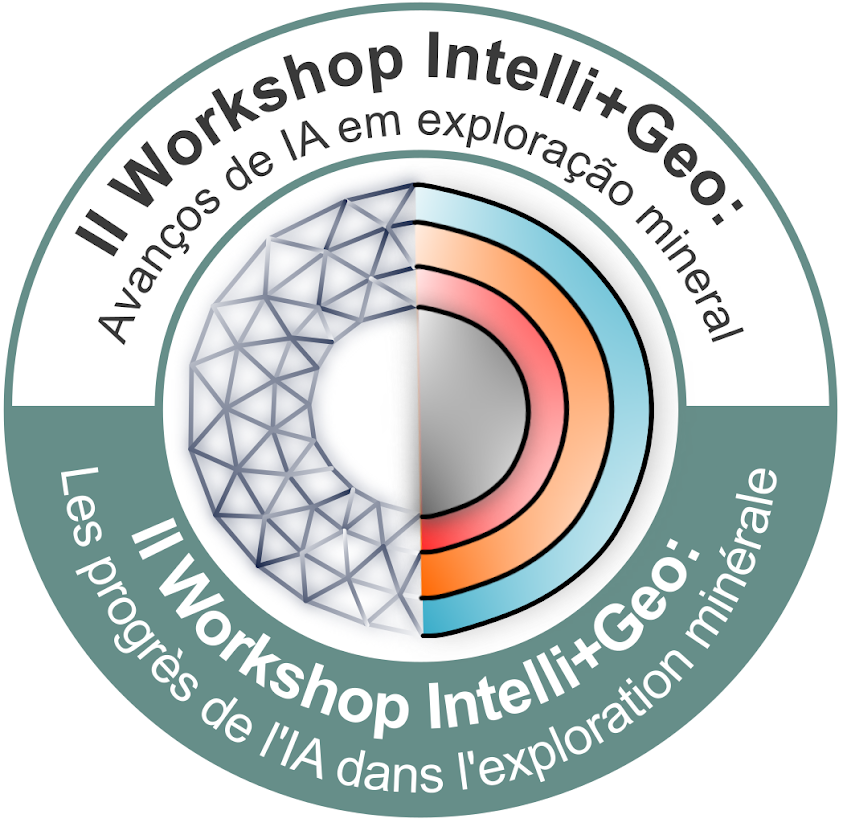
\includegraphics[scale=0.05]{./logo.png}
            \end{flushleft}
            \begin{flushright}
                \center Patrocínio / \textit{Sponsorship}\\
                \vspace{-0.5cm} 
                \center \rule{0.25\textwidth}{0.4pt} \thepage \\
                \vspace{0.1cm} 
                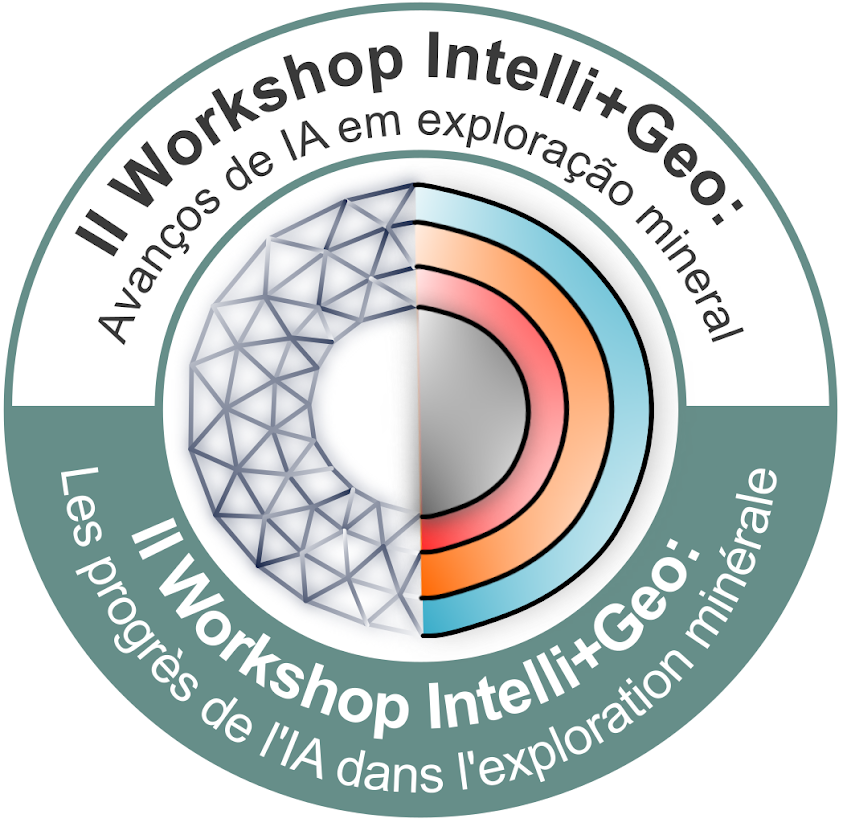
\includegraphics[scale=0.05]{./logo.png}
                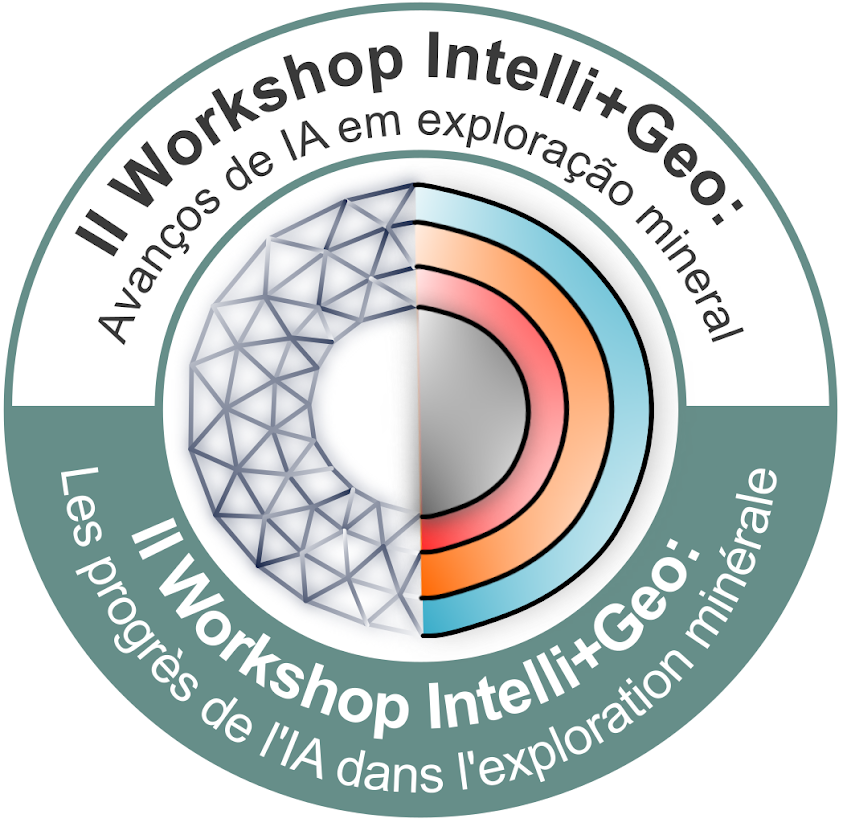
\includegraphics[scale=0.05]{./logo.png}
            \end{flushright}
        \end{multicols}
    }
}



\title{
    \vspace*{1.5cm}
    \small \textbf{Da Terra ao Código: Integrando Dados Geológicas a Inteligência Computacional}\\
    \vspace{0.25cm}
    \small Gabriel Góes Rocha de Lima\\
    \vspace{0.25cm}
    \small Universidade de São Paulo, IGc\\
    \vspace{0.25cm}
    \small gabrielgoes@usp.br
    
}
\date{}
\maketitle

% Transformar texto em itálico
\newcommand{\italic}[1]{\textit{#1}}

\vspace{-2.0cm}

\par{Este projeto propõe a criação de uma abordagem integrada que combina bases de dados
geológicas a modelos de classificação litológica, visando avançar nas
metodologias de exploração mineral. Em fase conceitual, esta iniciativa busca estabelecer
uma colaboração multidisciplinar entre geocientistas e programadores, visando
desenvolver uma plataforma que permita a geração e atualização dinâmica de mapas
litológicos preditivos. Central para este empreendimento é o desenvolvimento de um
sistema que, ao integrar dados geológicos precisos com algoritmos de aprendizado de
máquina, possibilite a criação de mapas com uma acurácia aprimorada ao longo do tempo.
Este processo iterativo de aperfeiçoamento se baseia na inclusão contínua de novos dados
e na avaliação rigorosa de métricas de desempenho, tais como precisão, sensibilidade
(\italic{recall}), e valor F1, além da análise da área sob a curva ROC. Estas métricas são vitais
para assegurar a confiabilidade e aplicabilidade das classificações do sistema no campo
da exploração mineral. A infraestrutura tecnológica proposta para sustentar tal sistema
envolve a utilização do PostgreSQL e da extensão PostGIS, criando um fundamento sólido
para o gerenciamento e análise eficientes de dados geoespaciais. Essa configuração não
apenas suportará as análises complexas requeridas pelo projeto mas também permitirá
uma gestão dinâmica e sistemática dos dados. Além disso, a implementação de folhas
cartográficas no processo de mapeamento assegurará que o sistema seja capaz de
adaptar-se a uma ampla gama de contextos geológicos, melhorando a classificação de
litologias e identificação de locais com potencial de mineralização. Adicionalmente, o
projeto aspira expandir suas capacidades para incluir a geração de mapas prospectivos
minerais preditivos. Este avanço significativo tem o potencial de transformar a exploração
mineral, indicando áreas com elevado potencial de mineralização e, consequentemente,
promovendo uma exploração mais eficiente e direcionada. Ao apresentar esta proposta
inovadora no \italic{II Workshop Intelli+Geo}, visa-se não apenas fomentar um debate
enriquecedor sobre as fronteiras entre geociências e tecnologia da informação, mas
também demonstrar a viabilidade e o potencial impactante do conceito através de um
esboço de protótipo funcional. Este protótipo inicial, ainda em estágios rudimentares de
desenvolvimento, serve como prova de conceito, ilustrando a capacidade de integração de
dados geológicos e modelos de classificação para aprimorar a precisão e eficácia na
exploração mineral. A partilha desta fase preliminar com especialistas e acadêmicos do
setor procura não apenas validar a abordagem proposta, mas também angariar
colaborações estratégicas e \italic{insights} valiosos que contribuam para a evolução do projeto.}

\end{document} % fim do documento
